\documentclass[hyperref={pdfpagemode=UseOutlines},xcolor=dvipsnames]{beamer}
\usetheme[secheader]{Madrid}
\setbeamertemplate{caption}[numbered]

\usepackage[utf8]{inputenc} % unicode support
\usepackage{lmodern} % enable different font sizes
\usepackage{stmaryrd} % more symbols
\usepackage{amsmath,amsfonts,amssymb} % maths
\usepackage{mathtools} % maths operators
\usepackage{faktor} % quotient rings
\usepackage{graphicx} % graphics
\usepackage{float} % define floating objects like tables or figures
\usepackage{tikz} % draw images
\usepackage{booktabs} % table lines
\usepackage{url} % website links
\usepackage{csquotes} % quotes
\usepackage{multirow} % multirows for tables
\usepackage{multicol} % multicolumns for itemize
\usepackage[backend=biber,sorting=none,style=alphabetic]{biblatex} % references
\usepackage[linesnumbered, ruled]{algorithm2e} % algorithm package
\usepackage{aliascnt} % alias counter package

% macros
\setbeamertemplate{itemize subitem}[triangle]
% \newcommand{\<command>}[<parameters>]{<formula>}

% maths operators
\DeclareMathOperator{\ord}{ord}
\DeclareMathOperator{\poly}{poly}
\DeclarePairedDelimiter{\floor}{\lfloor}{\rfloor}
\DeclarePairedDelimiter{\abs}{\lvert}{\rvert}
\DeclarePairedDelimiter{\norm}{\lVert}{\rVert}
\DeclarePairedDelimiter{\paren}{(}{)}
\DeclarePairedDelimiter{\bkt}{[}{]}
\DeclarePairedDelimiter{\set}{\{}{\}}
\DeclarePairedDelimiter{\innerprod}{\langle}{\rangle}

% counters
\newcounter{savenumi}
\newcommand{\seti}{\setcounter{savenumi}{\value{enumi}}}
\newcommand{\conti}{\setcounter{enumi}{\value{savenumi}}}
\newaliascnt{mycounter}{figure} % let "counter" be an alias for "figure"
\makeatletter
	\let\c@table=\c@mycounter % use mycounter for tables
	\let\c@algocf=\c@mycounter % use mycounter for algocf
\makeatother
\newcommand\addtag{\refstepcounter{mycounter} \tag{\themycounter}} % use mycounter for equations

% algorithms
\SetKwInOut{Initialization}{Initialization}

% url
\def\UrlBreaks{\do/\do-}

% bibliography
\addbibresource{references.bib}

% title page before section
\AtBeginSection[]
{
	\begin{frame}
		\vfill
		\centering
		\begin{beamercolorbox}[sep=8pt,center,shadow=true,rounded=true]{title}
			\usebeamerfont{title} Section~\thesection:~\secname
		\end{beamercolorbox}
		\vfill
	\end{frame}
}

\AtBeginSubsection[]
{
	\begin{frame}
		\tableofcontents[sections=\thesection,currentsubsection]
	\end{frame}
}

% tikz
\usetikzlibrary{shapes.geometric, arrows}
\tikzstyle{arrow} = [thick,->,>=stealth]
\tikzstyle{bluerect} = [rectangle, minimum width=3em, minimum height=2em, text centered, draw=black, fill=Cerulean]
\tikzstyle{yellowrect} = [rectangle, minimum width=3em, minimum height=2em, text centered, draw=black, fill=Goldenrod]
\tikzstyle{greenrect} = [rectangle, minimum width=3em, minimum height=2em, text centered, draw=black, fill=ForestGreen]
\tikzstyle{purplerect} = [rectangle, minimum width=3em, minimum height=2em, text centered, draw=black, fill=Orchid]

\title{Beamer Template}
\author{Sim Jun Jie}

\begin{document}

\frame{\titlepage}

\begin{frame}[allowframebreaks]{Contents}
	\tableofcontents[hideallsubsections]
\end{frame}

\section{Slide Design and Formatting}
\begin{frame}{Colored Text}
	\begin{itemize}
		\item {\color{red} red}
		\item {\color{blue} blue}
		\item {\color{magenta} magenta}
		\item {\color{Green} Green}
		\item {\color{BurntOrange} BurntOrange}
		\item {\color{Dandelion} Dandelion}
		\item {\color{Orchid} Orchid}
		\item {\color{Cerulean} Cerulean}
		\item {\color{Goldenrod} Goldenrod}
		\item {\color{ForestGreen} ForestGreen}
	\end{itemize}
\end{frame}

\section{Images and Figures}
\begin{frame}{Image}
	\begin{figure}
		\begin{minipage}{\textwidth}
			\centering
			\includegraphics[width=0.8\textwidth,height=15em]{stream.jpg}
			\caption{Caption for image}
			\label{fig:sample_image}
		\end{minipage}
	\end{figure}
\end{frame}

\begin{frame}{Tikz Figure}
	\begin{figure}
		\centering
		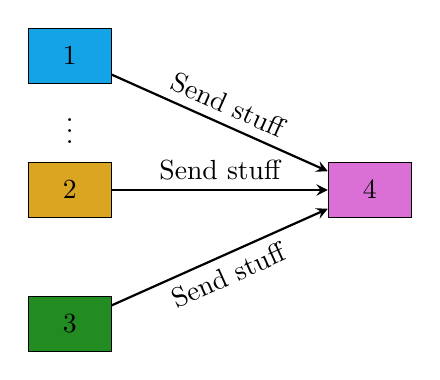
\begin{tikzpicture}
			\node (S1) [bluerect] {$1$};
			\node (S2) [yellowrect, below of=S1, yshift=-2em] {$2$};
			\node (S3) [greenrect, below of=S2, yshift=-2em] {$3$};
			\node (S4) [purplerect, right of=S2, xshift=8em] {$4$};

			\path (S1) -- node[auto=false]{$\vdots$} (S2);
			\draw [arrow] (S1) -- node[midway,above,sloped]{Send stuff}(S4);
			\draw [arrow] (S2) -- node[midway,above]{Send stuff}(S4);
			\draw [arrow] (S3) -- node[midway,below,sloped]{Send stuff}(S4);
		\end{tikzpicture}
		\caption{Tikz Figure}
		\label{tikz-figure}
	\end{figure}
\end{frame}

\section{Tables}
\begin{frame}{Tables}
	\begin{table}[H]
		\centering
		\caption{This is a table.}
		\label{table1}
		\begin{tabular}{lcccc}
			\toprule
			& col $1$ & col $2$ & col $3$ & col  $4$ \\
			\midrule
			row $1$ & $(1,1)$ & $(1,2)$ & $(1,3)$ & $(1,4)$ \\
			row $2$ & $(2,1)$ & $(2,2)$ & $(2,3)$ & $(2,4)$ \\
			row $3$ & $(3,1)$ & $(3,2)$ & $(3,3)$ & $(3,4)$ \\
			\bottomrule
		\end{tabular}
	\end{table}
\end{frame}

\section{Algorithms}
\begin{frame}{Sample Algorithm}
	\begin{center} % figure environment not needed
		\resizebox{0.8\textwidth}{!}{
			\begin{algorithm*}[H]
				\caption{This is an algorithm.}
				\label{algo1}
				\KwIn {Some inputs}
				\KwOut {Some outputs}
				\Initialization {Some variables}

				\While {condition not met}
				{
					Some code\;
					Some more code\; \label{line1}
				}
				\For {$i = 0$ \KwTo $k$}
				{
					\uIf {some condition holds}
					{
						Do some magic\;
					}
					\Else
					{
						\Return $m$\;
					}
				}
			\end{algorithm*}
		}
	\end{center}
\end{frame}

\section{Citation and Cross-References}
\begin{frame}{Citation and Cross-References}
	\begin{itemize}
		\item Cite stuff with \cite{article} and \cite{misc}.
		\item Combine citations like \cite{book,incollection}.
		\item Cross-Reference to tables with Table~\ref{table1} and figures with Figure~\ref{tikz-figure}.
		\item Note that \texttt{cleveref} does not work with \texttt{beamer}.
	\end{itemize}
\end{frame}

\begin{frame}
	\centering \Large
	\emph{Thank you}
\end{frame}

\section{References}
\begin{frame}[allowframebreaks]{References}
	\nocite{*}
	\printbibliography
\end{frame}

\end{document}
